\documentclass{DateStructure}

\SubjectName{最小生成树问题}
\CollegeName{理学院}
\Major{信息与计算科学}
\GroupNumber{第十六组}
\StudentA{20071226}{童繁}{流程图}
\StudentB{20071227}{王瀚功}{数据}
\StudentC{20071228}{王赛豪}{文案}
\StudentD{20071229}{吴政豪}{调试}
\StudentE{20071230}{武琦}{代码}

\begin{document}
\makecover
\newpage
\thispagestyle{empty}
\tableofcontents   
\newpage
\setcounter{page}{1}  

\section{需求分析}
\begin{itemize}
\item[(1)]利用普利姆算法求网的最小生成树;
\item[(2)]以文本形式输出生成树中各条边以及他们的权值。
\end{itemize}

\section{项目亮点}
\begin{itemize}
\item[(1)]使用system来命令Graphviz绘制网以及最小生成树的图,更加直观地展现了结果。
\item[(2)]本程序考虑了多种错误输入情况,具有很高的鲁棒性。
\item[(3)]设计了手动输入网和自动生成网两种功能,满足不同的需求。
\end{itemize}
\section{概要设计}
普里姆算法在找最小生成树时,将顶点分为两类,一类是在查找的过程中已经包含在树中的(假设为A类),剩下的是另一类(假设为B类)。\par
对于给定的连通网,起始状态全部顶点都归为B类。在找最小生成树时,选定任意一个顶点作为起始点,并将之从B类移至A类;然后找出B类中到A类中的顶点之间权值最小的顶点,将之从B类移至A类,如此重复,直到B类中没有顶点为止。所走过的顶点和边就是该连通图的最小生成树,算法运行的时间复杂度为$O(n^2)$。\par
\section{详细设计}
\subsection{判断顶点在二维数组中的位置}	
\begin{lstlisting}[language=c,caption={LocateVex}]
int LocateVex(MGraph G,VertexType v)//判断顶点在二维数组中的位置
{
    for(int i=0;i<G.vexnum;i++)
    {
        if(G.vexs[i]==v) return i;
    }
    return -1;
}
\end{lstlisting}
\subsection{创建无向网}
\begin{figure}[H] 
\centering
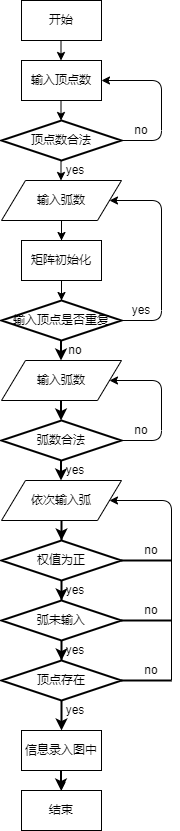
\includegraphics[width=100pt]{流程.png}
\caption{创建流程}
\end{figure}
\begin{lstlisting}[language=c,caption={Create}]
void Create(MGraph *G)//创建无向网
{
    int i,j,k,v1,v2,w,m,n,flag;
    A:printf("请输入顶点数:");scanf("%d",&(G->vexnum));
    if(G->vexnum<=1||G->vexnum>30) {printf("顶点数输入错误!\n");goto A;}//顶点个数不合法
    B:flag=0;
    for(i=0;i<G->vexnum;i++)//输入顶点
    {
        printf("请输入第%d个顶点:",i+1);
        scanf("%d",&(G->vexs[i]));
        for(j=0;j<G->vexnum;j++)//矩阵初始化
        {
            G->arcs[i][j].adj=INFINITY;
            G->arcs[i][j].info=NULL;
        }
    }
    for(i=0;i<G->vexnum;i++)//顶点输入重复
    {
        for(j=i+1;j<G->vexnum;j++)
        {
            if(G->vexs[i]==G->vexs[j]) {flag=1;break;}
        }
    }
    if(flag) {printf("顶点输入重复!\n");goto B;}
    C:printf("请输入弧数:");scanf("%d",&(G->arcnum));
    if(G->arcnum<1||G->arcnum>G->vexnum*(G->vexnum-1)/2) {printf("弧数不合法!\n");goto C;}//弧数不合法
    printf("请依次输入弧(顶点A 顶点B 弧值):\n");
    for(k=0;k<G->arcnum;k++)
    {
        D:flag=0;
        printf("第%d条弧:",k+1);
        scanf("%d %d %d",&v1,&v2,&w);
        for(i=0;i<G->arcnum;i++)//弧已输入
        {
            if(v1==v[i][0]&&v2==v[i][1]||v1==v[i][1]&&v2==v[i][0])
            {
                flag=1;
                break;
            }
        }
        if(flag) {printf("%d-%d的弧已输入!\n",v1,v2);goto D;}
        if(w<=0) {printf("弧值输入错误!\n");goto D;}//弧值非正
        m=LocateVex(*G,v1);n=LocateVex(*G,v2);
        if(m==-1||n==-1) {printf("顶点输入错误!\n");goto D;}
        if(m==n) {printf("顶点%d重复!\n",v1);goto D;}
        v[k][0]=v1;v[k][1]=v2;v[k][2]=w;
        G->arcs[n][m].adj=w;
        G->arcs[m][n].adj=w;
    }
}
\end{lstlisting}
\subsection{自动创建无向网}
用户首先输入顶点数n,在检验合法性后自动生成从1到n的自然数顶点;然后用户输入网中边的权最大值,程序生成$\frac{n(n-1)}{2}$条边及对应的权值,这样就创建了一个顶点数为n的随机的无向网。
\begin{lstlisting}[language=c,caption={create}]
void create(MGraph *G)//自动创建无向网
{
    int a,b,i,j,k=0,m,n;
    A:printf("请输入顶点数:");scanf("%d",&(G->vexnum));
    if(G->vexnum<=1||G->vexnum>30) {printf("顶点数输入错误!\n");goto A;}//顶点个数不合法
    B:printf("请输入生成随机数最大值:");scanf("%d",&b);
    if(b<=0||b>INFINITY) {printf("输入超出范围!");goto B;}
    for(i=0;i<G->vexnum;i++)
    {
        G->vexs[i]=i+1;
        for(j=0;j<G->vexnum;j++)//矩阵初始化
        {
            G->arcs[i][j].adj=INFINITY;
            G->arcs[i][j].info=NULL;
        }
    }
    G->arcnum=G->vexnum*(G->vexnum-1)/2;
    for(i=1;i<=G->vexnum;i++)
    {
        for(j=i+1;j<=G->vexnum;j++)
        {
            a=rand()%(b+1)+1;     //生成1~b之间的随机整数
            m=LocateVex(*G,i);n=LocateVex(*G,j);
            v[k][0]=i;v[k][1]=j;v[k][2]=a;k++;
            G->arcs[n][m].adj=a;
            G->arcs[m][n].adj=a;
        }
    }
}
\end{lstlisting}
\subsection{找出权值最小的边的数组下标}
\begin{lstlisting}[language=c,caption={minimum}]
int minimum(MGraph G,closedge c)//从辅助数组中找出权值最小的边的数组下标
{
    int i,min=INFINITY,index=-1;
    for(i=0;i<G.vexnum;i++) 
    {
        if(c[i].lowcost>0&&c[i].lowcost<min)
        {
            min=close[i].lowcost;
            index=i;
        }
    }
    return index;
}
\end{lstlisting}
\subsection{普里姆算法}
将绘制图的程序内嵌到普利姆算法中,创建一个graphviz文件,在使用普利姆算法输出最小生成树时,首先将最小生成树的边写入,边的颜色为蓝;之后写入其余的边,边无特定颜色。这样画出的图即包含整个网,又能明显看出最小生成树,同时在生成的graphviz文件中也可以看到所有的信息,一举三得。
\begin{lstlisting}[language=c,caption={MiniSpanTree\_PRIM}]
void MiniSpanTree_PRIM(MGraph G,VertexType u)//普里姆算法
{
    int i,j,k,m,num=G.arcnum,n[G.vexnum-1][2];
    char name[100],file[100],command[200]="dot ";
    printf("请输入文件名:");
    fflush(stdin);gets(name);strcpy(file,name);
    strcat(file,".png");strcat(name,".gv");
    FILE *fp=fopen(name,"w+");
    fprintf(fp,"graph\n{\n//best\n");
    k=LocateVex(G,u);
    for(i=0;i<G.vexnum;i++)//辅助数组初始化
    {
        if(i!=k)
        {
            close[i].adjvex=k;
            close[i].lowcost=G.arcs[k][i].adj;
        }
    }
    close[k].lowcost=0;//初始
    for(i=1;i<G.vexnum;i++)//选择其余G.vexnum-1个顶点
    {
        k=minimum(G,close);//求出T的下一个节点:第k顶点
        m=close[k].adjvex;
        n[i-1][0]=G.vexs[m];n[i-1][1]=G.vexs[k];
        fprintf(fp,"v%d--v%d [label=\"%d\" color=blue];\n",G.vexs[m],G.vexs[k],G.arcs[m][k].adj);//输出生成树的边
        close[k].lowcost=0;//第k顶点并入U集
        for(j=0;j<G.vexnum;j++)
        {
            if(G.arcs[k][j].adj<close[j].lowcost)//新顶点并入U后重新选择最小边
            {
                close[j].adjvex=k;
                close[j].lowcost=G.arcs[k][j].adj;
            }
        }
    }
    for(i=0;i<num;i++)//筛选其他弧
    {
        for(j=0;j<G.vexnum-1;j++)
        {
            if(v[i][0]==n[j][0]&&v[i][1]==n[j][1]||v[i][0]==n[j][1]&&v[i][1]==n[j][0])
            {
                for(m=i;m<num;m++)
                {
                    for(k=0;k<3;k++)
                        v[m][k]=v[m+1][k];
                }
                num--;
                i--;
                break;
            }
        }
    }
    fprintf(fp,"//other\n");
    for(i=0;i<num;i++)//输出其他弧
        fprintf(fp,"v%d--v%d [label=\"%d\"];\n",v[i][0],v[i][1],v[i][2]);
    printf("成功生成最小生成树!\n");
    fprintf(fp,"}");
    fclose(fp);
    strcat(command,name);strcat(command," -Ksfdp -Tpng -o ");strcat(command,file);
    system(command);
}
\end{lstlisting}

\section{用户手册}
\subsection{界面}
\begin{figure}[H] 
\centering
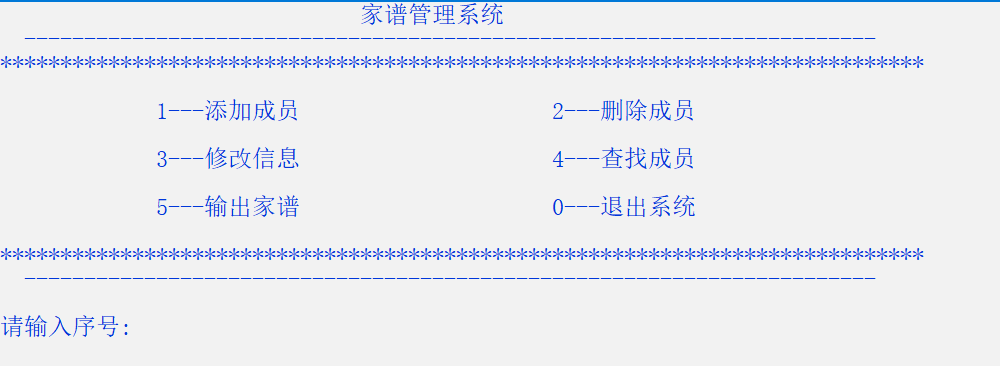
\includegraphics[width=200pt]{界面.png}
\caption{用户界面}
\end{figure}
\subsection{手动输入}
\begin{figure}[H] 
\centering
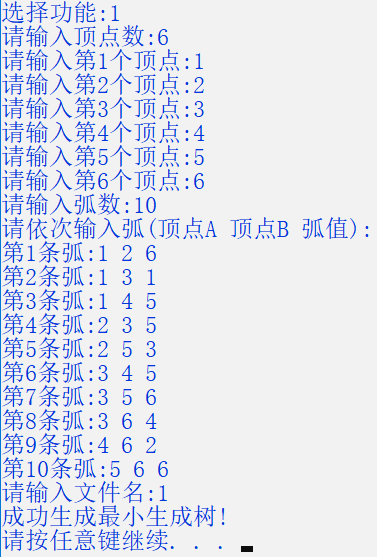
\includegraphics[width=200pt]{输入1.png}
\caption{手动输入一张网}	
\end{figure}
\begin{figure}[H] 
\centering
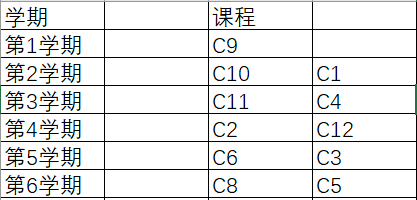
\includegraphics[width=\linewidth]{1.png}
\caption{功能1的最小生成树}	
\end{figure}
\lstinputlisting{1.gv}
\subsection{自动生成}
\begin{figure}[H] 
\centering
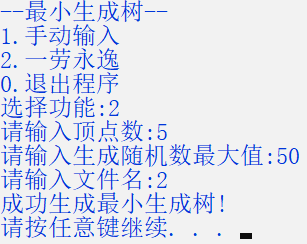
\includegraphics[width=200pt]{输入2.png}
\caption{自动生成一张网}	
\end{figure}
\begin{figure}[H] 
\centering
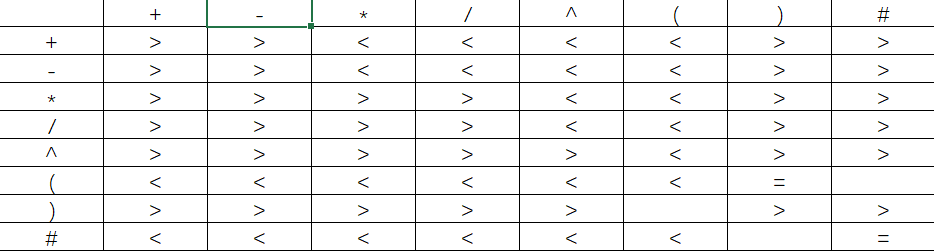
\includegraphics[width=\linewidth]{2.png}
\caption{功能2的最小生成树}	
\end{figure}
\lstinputlisting{2.gv}


\section{心得体会}
这次课程设计的心得体会通过实践我们的收获如下:\par
1.在这次的最小生成树课程设计的过程中,我们更深刻地了解了普利姆算法的特点与用法。\par
2.学会了使用Graphviz。\par
3.由于这次的课程设计相对简单,因此增强了程序的鲁棒性,为以后的Debug提供了思路。

\newpage 
\section{附录}
\lstinputlisting[language=C]{main.c}

\end{document}
